\section{Systemarkitektur}
Med udgangspunkt i usecasene er systemets funktionalitet forsøgt brudt ned i mindre logiske blokke. Disse skal dække over betjening af systemet, detektering af vinflaske og åbningen af denne. På baggrund af disse krav er BDD'et i figur \ref{BDD_WinePrep} udarbejdet.

\begin{figure}[H]
	\centerline{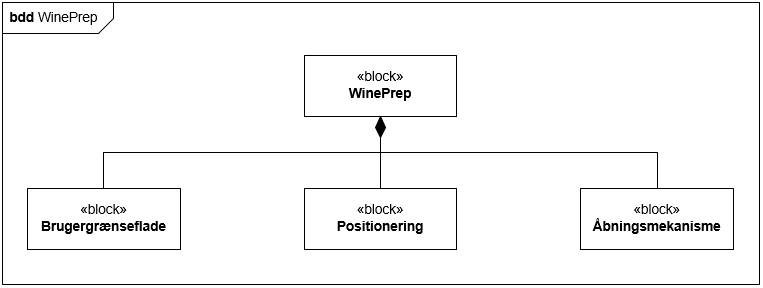
\includegraphics[scale=0.33]{tex/Arkitektur/Diagrammer/BDD_WinePrep}}
	\caption{BDD for WinePrep}
	\label{BDD_WinePrep}
\end{figure}

\textbf{Brugergrænsefladen} betjenes af bruger og initierer usecasene som beskrevet i Krav.
\\
\textbf{Positionering} finder vinflaskens position og indstiller WinePrep, så den er klar til at åbne vinflasken.
\\
\textbf{Åbningsmekanismen} fjerner proppen fra flasken og dispenserer denne.

For at forstå den interne funktionalitet og kompleksitet i blokkene \textbf{Positionering} og \textbf{Åbningsmekanisme} er disse brudt yderligere ned.

\subsection{Positionering}
For at finde flaskens position er det nødvendigt at have et modul, som skal stå for selve detekteringen af denne flaske, samt et modul, som står for løbende at ændre den 

\begin{figure}[H]
	\centerline{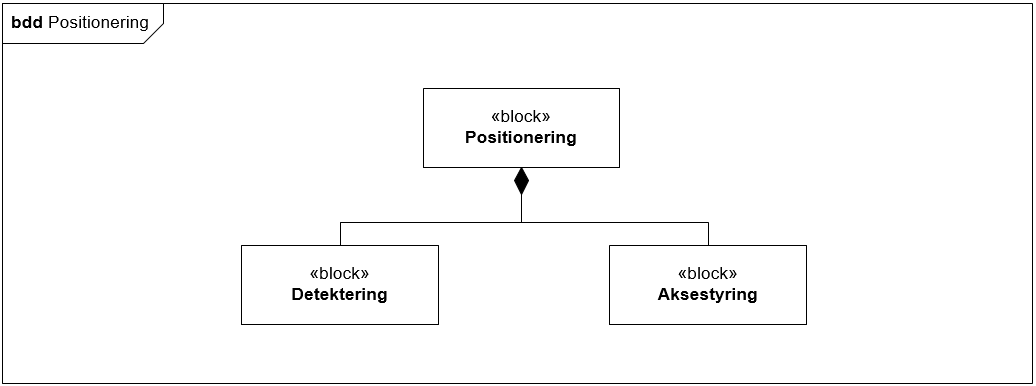
\includegraphics[scale=0.33]{tex/Arkitektur/Diagrammer/BDD_Positionering}}
	\caption{BDD for Positionering}
	\label{BDD_Positionering}
\end{figure}